\documentclass{article}
\usepackage{graphicx,amsmath}
\title{CosmoCalc: an Excel Add-In for cosmogenic nuclide
calculations \\ {\normalsize manuscript submitted to G-Cubed}}
\author{Pieter Vermeesch 
\date{}
\footnote{Institute of Isotope Geology and Mineral Resources, ETH-Z\"{u}rich,
cosmocalc@gmail.com, http://cosmocalc.googlepages.com}
}
\begin{document}
\maketitle
\begin{abstract}
  As dating methods using Terrestrial Cosmogenic Nuclides (TCN) become
  more popular, the need  arises for a general-purpose and easy-to-use
  data reduction software.  The  CosmoCalc Excel add-in calculates TCN
  production  rate  scaling  factors  (using  Lal,  Stone,  Dunai  and
  Desilets  methods); topographic,  snow  and self-shielding  factors;
  exposure  ages, erosion rates  and burial  ages; and  visualizes the
  results on banana-style plots.  It uses an internally consistent TCN
  production  equation  that is  based  on  the quadruple  exponential
  approach of  [Granger and  Smith, 2000, NIM-B  (172) pp.   824-828]. 
  CosmoCalc was designed to be as user-friendly as possible.  Although
  the  user-interface is extremely  simple, the  program is  also very
  flexible, and  nearly all default  parameter values can be  changed. 
  To facilitate the comparison of  different scaling factors, a set of
  converter  tools is provided,  allowing the  user to  easily convert
  cut-off   rigidities  to   magnetic   inclinations,  elevations   to
  atmospheric depths and  so forth.  Because it is  important to use a
  consistent set  of scaling factors  for the sample  measurements and
  the  production  rate   calibration  sites,  CosmoCalc  defines  the
  production  rates implicitly,  as  a function  of  the original  TCN
  concentrations of the calibration  site.  The program is best suited
  for  $^{10}$Be,  $^{26}$Al,  $^{3}$He  and  $^{21}$Ne  calculations,
  although  basic functionality  for  $^{36}$Cl and  $^{14}$C is  also
  provided.  CosmoCalc can be downloaded along with a set of test data
  from \texttt{http://cosmocalc.googlepages.com}
\end{abstract}

\section{Introduction}\label{sec:intro}
The  first  applications   of  Terrestrial  Cosmogenic  Nuclide  (TCN)
geochronology appeared  about 20 years ago (Kurz,  1986; Nishiizumi et
al., 1986; Phillips  et al., 1986).  The method  has rapidly developed
since  those  early  days,  truely revolutionizing  geomorphology  and
related fields in the process.   TCN dating is no longer a specialized
tool used by a small group of experienced users, but has found an ever
growing base  of users who are  not necessarily familiar  with all the
details of the method.  Today we are facing a paradoxal situation.  On
the one hand, a  better understanding of cosmogenic nuclide production
systematics has improved the accuracy  of TCN dating. But on the other
hand,  many  users  of  the  method  may be  less  familiar  with  its
intricacies than  was the case  in the pioneering days.   An important
example  of this  situation is  that  of the  production rate  scaling
factors.   In a  landmark  paper,  Lal (1991)  presented  a method  to
calculate  cosmogenic  nuclide  production  rates  as  a  function  of
latitude and elevation.  Lal's scaling factors are elegant and easy to
use, but overestimate  the importance of muons and  are only valid for
standard atmosphere.   Later authors introduced  several improvements,
incorporating  atmospheric   effects  and  improved   muon  production
systematics.  The  scaling factors of Stone (2000),  Dunai (2000), and
Desilets et al. (2003, 2006)  more accurately represent the scaling of
cosmogenic nuclide  production rates with latitude  and elevation, but
the increased sophistication of these  methods is an obstacle to their
widespread use.
\\

CosmoCalc is  an add-in  to MS-Excel developed  with the  intention to
alleviate this problem.  The CosmoCalc interface was designed to be as
user friendly and easy-to-use as possible.  Default parameters are set
so  that  beginning  users only  have  to  make  a minimal  number  of
decisions. At the same time, all the default parameters can be changed
so that  CosmoCalc is highly  customizable and also  experienced users
should find it useful.  The program as well as a spreadsheet with test
data    can    be    downloaded    from    the    CosmoCalc    website
(\texttt{http://cosmocalc.googlepages.com}),   which   also   provides
detailed installation instructions.  The add-in requires MS-Excel 2000
or  higher. Because of  small differences  between the  MS-Windows and
Apple  OS-X implementations of  Excel, two  versions of  CosmoCalc are
provided.  The  functionality of  both programs is  the same,  but the
Macintosh version is significantly slower than the PC-version.
\\

After installing the CosmoCalc  add-in, a toolbar menu appears (Figure
\ref{fig:CosmoMenu}) that  guides the user through  the data reduction
and closely follows the outline of this paper:

\begin{itemize}
\item{Production rate scaling factors} (Section \ref{sec:scaling})
  \begin{itemize}
  \item Lal (1991)
  \item Stone (2000)
  \item Dunai (2000)
  \item Desilets and Zreda (2003)
  \item Desilets et al. (2006)
  \end{itemize}
\item{Shielding corrections} (Section \ref{sec:shielding})
  \begin{itemize}
  \item Topographic shielding
  \item Self shielding
  \item Snow shielding
  \end{itemize}
\item{Banana plots} (Section \ref{sec:banana})
  \begin{itemize}
  \item $^{26}$Al-$^{10}$Be
  \item $^{21}$Ne-$^{10}$Be 
  \end{itemize}
\item{Age/erosion rate calculations} (Section \ref{sec:age})
  \begin{itemize}
  \item Single nuclide: exposure age and erosion rate calculations for 
    $^{26}$Al, $^{10}$Be, $^{21}$Ne, $^{3}$He, $^{36}$Cl and $^{14}$C
  \item Two nuclides: simultaneous calculation of (burial or exposure)
    age and erosion rate.
  \end{itemize}
\item{Converters} (Section \ref{sec:converter})
  \begin{itemize}
  \item Convert elevation to  atmospheric pressure or -depth and back,
    under standard and Antarctic atmosphere.
  \item  Convert  geomagnetic   latitude  to  -inclination  or  cutoff
    rigidity and back.
  \end{itemize}
\item{Settings: customizing CosmoCalc} (Section \ref{sec:settings})
  \begin{itemize}
  \item Specify  TCN production rate calibration sites
  \item Specify the relative importance of various production pathways
  \end{itemize}
\end{itemize}

The  following   sections  will  provide  more   details  about  these
calculations.  Thus, the present paper serves as an abridged review of
TCN calculations, with  an emphasis on the numerical  methods that are
needed to solve the equations.   More details about the physics of TCN
production  are given  in  the  review article  of  Gosse and  Philips
(2001).   CosmoCalc  is  not  the  first computational  tool  for  TCN
calculations.  Useful alternatives are CHLOE, an Excel spreadsheet for
cosmogenic $^{36}$Cl calculations (Phillips and Plummer, 1996) and the
CRONUS-Earth     web-calculator     (Balco     and    Stone,     2007;
\texttt{http://hess.ess.washington.edu/math}).       CosmoCalc     was
developed  independently  from  these  other  tools,  except  for  its
topographic shielding  correction function, which  was translated into
VBA from  the Matlab code  of Balco and  Stone (2007).  The  reader is
strongly  encouraged  to  try  these  other  programs.   CosmoCalc  is
optimized  for $^{26}$Al,  $^{10}$Be, $^{21}$Ne  and $^{3}$He  dating. 
Because geomagnetic  field fluctuations and  thermal neutron reactions
are ignored,  results for  $^{36}$Cl and $^{14}$C  may be  inaccurate. 
CosmoCalc can be  used as an exploratory tool  for these nuclides, but
for more accurate  results, CHLOE or the spreadsheet of  Lifton et al. 
(2005) are recommended.

\begin{figure}[][h]
  \centering
  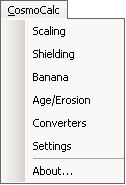
\includegraphics[height=2in]{2006GC001530-f01_orig.jpg}
  \caption{CosmoCalc's main menu guides the user through
    the data reduction and follows the outline of this paper.}
  \label{fig:CosmoMenu}
\end{figure}

\section{Production rate scaling factors}\label{sec:scaling}

In the  simplest case (no shielding  or burial), only  three pieces of
information are needed  to calculate an exposure age  or erosion rate:
TCN concentration, half-life and production rate. Production rates are
the  ``achilles heel''  of the  TCN method.   There exist  only  a few
calibration  sites where  TCN  production rates  are accurately  known
thanks  to  the availability  of  independent  age constraints  (e.g.,
Nishiizumi et al., 1989; Niedermann et al., 1994; Kubik et al., 1998).
These  production rates  are only  valid for  the  specific conditions
(latitude,  elevation, age)  of each  particular calibration  site. To
apply the  TCN method  to other field  settings, the  production rates
must be  scaled to a common  reference at sea level  and high latitude
(SLHL).   Up to  20\%  uncertainty is  associated  with this  scaling,
constituting the bulk of TCN age uncertainty.
\\

Although  several  efforts have  been  made  to  directly measure  TCN
production rate  scaling with latitude and  elevation using artificial
H$_2$O and  SiO$_2$ targets  (Nishiizumi et al.,  1996; Brown  et al.,
2000;  Graham et  al., 2007),  all currently  used scaling  models are
based on  neutron monitor surveys.   The oldest and still  most widely
used scaling model is that of  Lal (1991).  This model is a simple set
of polynomial equations giving the (spallogenic + muogenic) production
rate  relative  to SLHL  as  a  function  of geographic  latitude  and
elevation.  In  CosmoCalc, Lal's scaling factors can  be calculated by
simply selecting  two columns of  latitude (in degrees)  and elevation
(in meters) data and clicking ``OK''.
\\

Lal's scaling factors use elevation  as a proxy for atmospheric depth,
assuming a standard atmosphere approximation.  Stone (2000) noted that
this approximation is  not valid in certain areas,  such as Antarctica
and Iceland.   To avoid the  systematic errors caused by  the standard
atmosphere model, Stone (2000)  recast the polynomial equations of Lal
(1991) in  terms  of air  pressure  instead  of  elevation.  A  second
improvement of  the Stone (2000)  model is the independent  scaling of
TCN production by slow (negative)  muons (Heisinger et al., 2002).  In
spite  of this  added complexity,  the CosmoCalc  interface  for Stone
(2000) scaling factors  is identical to  that for Lal  (1991) scaling:
the  user  simply needs  to  provide two  columns  of  data, one  with
latitude and one  with air pressure (in mbar).  The scaling factors of
Stone  (2000) can  be different  for different  nuclides,  because the
importance of muons  depends on the nuclide of  interest. Because most
TCN production rate  calibration sites are {\it not}  located at SLHL,
it is crucially important to scale the production rates using the same
method as  the unknown  sample.  This is  exactly what  CosmoCalc does
when  the user  selects a  nuclide from  the scroll-down  menu  of the
scaling-form. Thus, the program ``forces''  the user to be consistent. 
The program comes  with a set of default  calibration sites, but these
can  be  changed.  Also  the  relative  importance  of the  production
pathways  (neutrons, slow  and  fast muons)  can  be changed  (Section
\ref{sec:settings}).
\\

Behind the scaling models of both  Lal (1991) and Stone (2000) lies an
extensive database of  neutron monitor measurements, ordered according
to geomagnetic  latitude. This ordering implies  that Earth's magnetic
field can be accurately approximated by a simple dipole. To avoid this
approximation, Dunai (2000) ordered the neutron monitor data according
to  geomagnetic  inclination,  which  also represents  the  non-dipole
field.   Just  like  Stone  (2000),  also  Dunai  (2000)  incorporates
separate  muon scaling and  atmospheric effects.  However, atmospheric
depth (g/cm$^2$) is used instead  of air pressure.  Using CosmoCalc it
is very easy to convert air pressure to elevation or atmospheric depth
and back (Section \ref{sec:converter}).
\\

Ultimately,  both  geomagnetic  latitude  and inclination  are  merely
proxies  for a  more  fundamental physical  quantity: the  geomagnetic
cutoff rigidity (R$_c$), which is the minimum momentum per unit charge
(in GV),  required for a primary  cosmic ray to reach  the atmosphere. 
Ordering the neutron monitor  data according to this parameter results
in yet another set of  scaling factors.  Unfortunately, at least three
different  methods for  calculating  R$_c$ exist  in  the literature.  
Dunai (2001) used a  database of horizontal magnetic field intensities
and  inclinations to  estimate  the cutoff-rigidity  of an  equivalent
axial  dipole  field, for  which  an  approximate analytical  solution
exists.  Desilets  and Zreda (2003)  used a model based  on trajectory
tracing of an axial dipole field, which is done by numerically testing
the feasibility of vertically incident anti-protons to travel from the
top of the atmosphere back into space.  Finally, Lifton et al.  (2005)
fit a  cosine function to  a database of geomagnetic  latitudes versus
trajectory  traced cutoff  rigidities  for the  1955  magnetic field.  
These authors consider the scatter  around their fit to be a realistic
estimator of the natural variability of R$_c$ at any given geomagnetic
latitude.
\\

In order  to avoid confusion, CosmoCalc currently  only implements one
of these three methods, namely that of Desilets and Zreda (2003).  The
scaling model of Desilets and Zreda (2003) makes a distinction between
slow and fast muons, each of which scales differently. In an update of
their model, Desilets  et al.  (2006) did a  neutron monitor survey at
low  latitudes, which  were  undersampled by  previous surveys.   This
resulted in a slightly different set of attenuation length polynomials
for  spallogenic reactions.   The method  of Desilets  et  al.  (2003,
2006) is  probably  the  most  accurate  of  all  the  scaling  models
implemented in CosmoCalc.  It is also the most complex model, but this
did  not change  the  user  interface.  Using  the  scaling models  of
Desilets et al.  (2003, 2006) is just as easy as that of Lal (1991) in
CosmoCalc.   Default  values for  the  relative  SLHL production  rate
contributions of neutrons,  slow and fast muons can  be changed in the
Settings menu  (Section \ref{sec:settings}).  
\\

The scaling  models of  Dunai (2001), Desilets  et al.   (2003, 2006),
Pigati and  Lifton (2004),  and Lifton et  al. (2005) are  a sensitive
function of magnetic field intensity and solar activity, both of which
are  poorly constrained  over geologic  time.  On  the one  hand, this
temporal variability is the biggest downside to R$_c$-based models for
long  exposures ($>$ 20  ka; Dunai,  2001).  On  the other  hand, such
models also offer the possibility  to correct for secular variation of
TCN production  rates for short  exposures. Instructions for  doing so
are given by Dunai (2001) and  Desilets et al. (2003), provided a {\it
  local}  record of paleomagnetic  intensity is  available.  Compiling
such a  record is  something for advanced  users and falls  beyond the
scope of  CosmoCalc.  The scaling  models of Pigati and  Lifton (2004)
and Lifton (2005) are accompanied by {\it global} datasets of magnetic
field intensity, polar wander and  solar activity and in principle, it
would  be  possible to  incorporate  these  datasets  into CosmoCalc.  
However,  because they  are very  large (4  and 7Mb,  respectively) in
comparison with CosmoCalc ($\sim$  500kb), the cost of including these
scaling  models  was  considered  too  high.   Therefore,  researchers
working with  $^{14}$C, where secular variation of  the magnetic field
is really crucial,  should use CosmoCalc only as  an exploratory tool,
and use the spreadsheets of Pigati and Lifton (2004) and Lifton et al.
(2005) for final calculations.

\section{Shielding corrections}\label{sec:shielding}

The  scaling  factors discussed  in  the  previous  section allow  the
calculation of  TCN production  rates at any  location on  the Earth's
surface, assuming  that the sample is  a slab of  zero thickness taken
from  a  horizontal  planar  surface.   If these  assumption  are  not
fulfilled, the  SLHL production rates  must be multiplied by  a second
set of correction factors, quantifying  the extent to which the cosmic
rays  were  blocked.    CosmoCalc  implements  three  such  correction
factors: topographic shielding, self shielding and snow cover.

\subsection{Topographic shielding}\label{sec:topo}

Two kinds  of topographic  shielding corrections can  be distinguished
for (a)  samples taken from  a tilted rather than  horizontal surface,
and  (b) samples  that  are  located in  the  vicinity of  topographic
irregularities.   CosmoCalc follows  the approach  of Balco  and Stone
(2007) (their Matlab function \texttt{skyline.m}) and treats these two
effects together using the following equation:

\begin{equation}
  \label{eq:topo}
  S_t = 1 - \int_0^{2 \pi}\frac{sin(h(\theta))^{3.5}}{2 \pi}d\theta
\end{equation}

With h($\theta$) the ``horizon''  in the azimuthal direction $\theta$,
i.e.   either the  elevation (in  radians)  of the  topography or  the
sloping sample surface, whichever is greatest.  Sometimes, an exponent
of 2.3  is used instead  of 3.5 in Equation  \ref{eq:topo} (Staudacher
and All\`{e}gre, 1993). CosmoCalc  treats this exponent as a variable,
which    can   be    changed   in    the   Settings    form   (Section
\ref{sec:settings}).    In   practice,   the  integral   of   Equation
\ref{eq:topo}  is  solved by  linear  interpolation  between a  finite
number  of  azimuth/elevation   measurements.   The  input  needed  by
CosmoCalc  is two  mandatory columns  of strike  and dip  (in degrees,
where the  strike is 90 degrees  less than the direction  of the dip),
followed  by  an  optional  series  of  topographic  azimuth/elevation
measurements (in degrees). There is no restriction on the total number
of measurements, provided they come in multiples of two.

\subsection{Self-shielding}\label{eq:self}

Cosmic  rays are  rapidly attenuated  as they  travel  through matter,
causing  TCN production  rates to  vary greatly  with depth  below the
rock/air  contact.  They  must be  integrated over  the  actual sample
thickness  and  scaled  to  the  surface production  rates  before  an
exposure  age can  be calculated.   Different reaction  mechanisms are
associated  with  different attenuation  lengths.   Gosse and  Philips
(2001) consider four kinds  of thickness corrections, for spallogenic,
thermal  and epithermal neutrons,  and muons.   Because self-shielding
corrections  are   generally  small,  CosmoCalc   considers  only  the
spallogenic neutron reactions:

\begin{equation}
  \label{eq:self}
  S_s = \frac{\Lambda_0}{\rho z} \left(1 - e^{-\frac{\rho  z}{\Lambda_0}}\right)
\end{equation}

with $\Lambda_0$  the spallogenic neutron  attenuation length (default
value  160 g/cm$^2$),  $\rho$  the rock  density  (default value  2.65
g/cm$^3$)  and  z  the  sample  thickness  (in  cm).   Neglecting  the
remaining  pathways   makes  little  difference,   with  the  possible
exception of $^{36}$Cl, because the latter can be strongly affected by
thermal neutron fluxes, which are currently ignored by CosmoCalc.

\subsection{Snow cover}

Perhaps the most popular and powerful application of TCN techniques is
the dating of glacial moraines  (e.g., Gosse et al., 1995; Sch\"{a}fer
et al., 1999).  These features are generally located at high latitudes
or elevations, where  snow cover poses a potential  problem.  The snow
correction  is  similar  to  the self-shielding  correction  with  the
important difference  that the  former is highly  variable with  time. 
Given  n (e.g.,  12 for  monthly or  4 for  seasonal)  measurements of
average snow  thickness z and  density $\rho$, CosmoCalc  computes the
snow correction factor S$_c$ as follows:

\begin{equation}
  \label{eq:snow}
  S_c = \frac{1}{n} \sum_{i=1}^{n} e^{-\frac{\rho(i)  z(i)}{\Lambda_0}}
\end{equation}

\section{Banana plots}\label{sec:banana}

Before calculating an exposure age or  erosion rate, it is a good idea
to  check if  the TCN  measurements are  consistent with  a  simple or
complex  exposure  history.   This  can  be  done  with  two  nuclides
(including at  least one radionuclide)  using a ``banana  plot'' (Lal,
1991).    CosmoCalc   accomodates    two   types   of   banana   plot:
$^{26}$Al-$^{10}$Be and $^{21}$Ne-$^{10}$Be.   Depending on whether or
not a sample plots above, below or inside the so-called ``steady-state
erosion island'' (Lal, 1991), one  can decide whether or not to pursue
the calculation of  an exposure age, erosion rate  or burial age.  For
the construction of the  banana plots and the age/erosion calculations
of Section  \ref{sec:age}, CosmoCalc implements a  modified version of
the ingrowth equation of Granger and Muzikar (2001):

\begin{equation}
  \label{eq:Nbanana}
N = P e^{- \lambda \tau}
\sum_{i=0}^3
\frac{F_i}{\lambda + \epsilon \rho / \Lambda_i}
\left( 1 - e^{- \left( \lambda + \epsilon \rho / \Lambda_i \right) t} \right)
\end{equation}

With  N  the nuclide  concentration  (atoms/g),  P  the total  surface
production  rate  (in atoms/g/yr)  at  SLHL,  $\tau$  the burial  age,
$\epsilon$  the erosion  rate, t  the exposure  age and  $\lambda$ the
radioactive  half-life  of  the  nuclide.   Equation  \ref{eq:Nbanana}
models TCN production by neutrons, slow  and fast muons by a series of
exponential approximations.   The first  term of the  summation models
TCN production by spallogenic  neutron reactions, the second and third
terms model slow  muons and the last term  approximates TCN production
by fast muons.  Thus,  $F_0,...,F_3$ are dimensionless numbers between
zero  and one, and  $\Lambda_0,...,\Lambda_3$ are  attenuation lengths
(g/cm$^2$).  The approach  of Granger et al.  (2000,  2001) was chosen
because of its flexibility.   For instance, neglecting muon production
can be easily implemented by setting $F_1,F_2$ and $F_3$ equal to zero
in Equation \ref{eq:Nbanana}.  CosmoCalc  uses Granger et al.'s (2000,
2001) recommended values of $F_0,...,F_3$ for $^{10}$Be and $^{26}$Al,
but also offers an  alternative choice of pre-set values approximating
either  the alternative  parameterization of  Schaller et  al. (2001),
neglecting the contribution of muons, or only using three exponentials
(for more details, see  Section \ref{sec:settings}). Banana plots with
non-zero muon contributions feature a characteristic cross-over of the
steady-state and  zero erosion  lines which is  absent when  muons are
neglected (Figure \ref{fig:compareBananas}).
\\

CosmoCalc's banana plots are normalized  to SLHL, meaning that the TCN
concentrations of each sample are  divided by the cumulative effect of
all their  correction factors, represented by  the ``effective scaling
factor'' S$_e$:

\begin{equation}
  \label{eq:Se}
S_e = S_t \times f(S)
\end{equation}

with

\begin{equation}
   \label{eq:S}
S = S_p \times S_s \times S_c
\end{equation}

where S$_p$ is  one of the production rate  scaling factors of Section
\ref{sec:scaling} and  S$_t$, S$_s$ and  S$_c$ are defined  in Section
\ref{sec:shielding}.  If  muon production  is neglected, then  S$_e$ =
S$_t$ $\times$  S$_p$ $\times$ S$_s$  $\times$ S$_c$. However,  in the
presence of muons, the effective scaling factor S$_e$ may deviate from
this value because the relative importance of the different production
mechanisms  changes as  a function  of age,  erosion  rate, elevation,
latitude,  sample thickness  and snow  cover.  The  exact form  of the
function f(S) will be defined  in Section \ref{sec:Se}.  Note that the
topographic shielding correction S$_t$ does not ``fractionate'' (i.e.,
change  the  fractions F$_0$,...,F$_3$  of)  the different  production
mechanisms  and is  placed outside  the scaling  function  f(S).  This
means  that,  strictly  speaking,  the TCN  concentrations  should  be
multiplied  by S$_t$  {\it prior}  to generating  a banana  plot.  The
input  required  by  CosmoCalc's   ``Banana''  function  are  (1)  the
composite  scaling  factor  S  for  the first  nuclide  ($^{26}$Al  or
$^{21}$Ne),   (2)   the   concentration  and   1$\sigma$   measurement
uncertainty  of  the  first  nuclide ($^{26}$Al  or  $^{21}$Ne),  both
multiplied by S$_t$, (3) S  for the second nuclide ($^{10}$Be) and (4)
the concentration and 1$\sigma$  measurement uncertainty of the second
nuclide  ($^{10}$Be), also multiplied  by S$_t$.   Because topographic
shielding corrections are generally small, the systematic error caused
by lumping  S$_t$ together with  the other correction factors  is very
small.   Therefore, if  S$_t$  $>$ $\sim$  0.95,  say, it  is safe  to
approximate  Equation \ref{eq:Se}  by S$_e$  = f(S$_t$  $\times$ S$_p$
$\times$   S$_s$  $\times$   S$_c$).   In   this  case,   the  nuclide
concentrations do not need to be pre-multiplied by S$_t$.
\\

\begin{figure}[htbp]
  \centering
a.  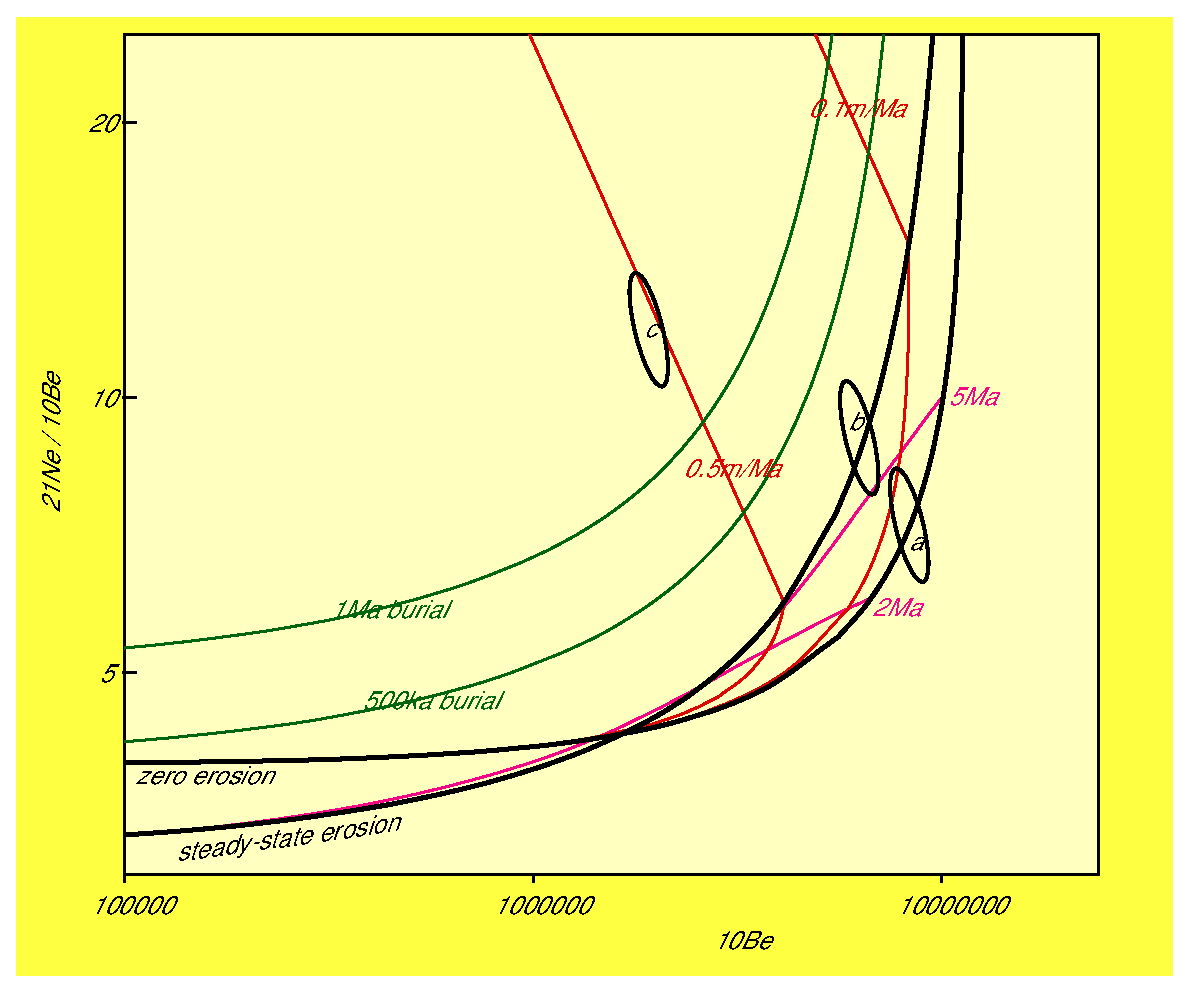
\includegraphics[width=0.7\textwidth]{2006GC001530-f02a_orig.eps}\\
b.  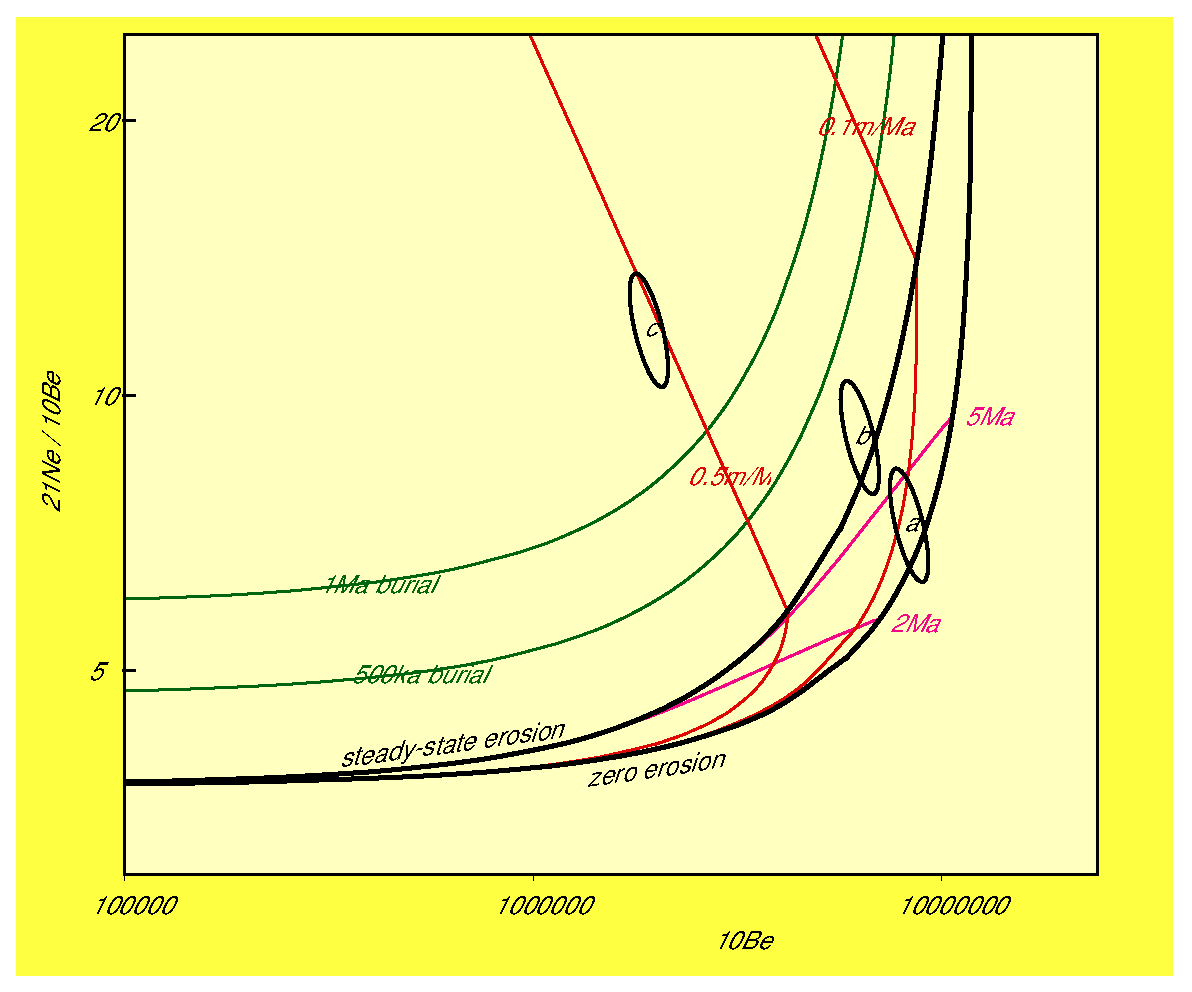
\includegraphics[width=0.7\textwidth]{2006GC001530-f02b_orig.eps}\\
  \caption{
    By using  the TCN  production equation of  Granger et  al.  (2000,
    2001;  Equation  \ref{eq:Nbanana}),  CosmoCalc's banana-plots  are
    very flexible.   Two examples of  $^{21}$Ne/$^{10}$Be-banana plots
    illustrate this  flexibility: a. with default  parameters as given
    by Granger  and Smith (2000)  and in Table \ref{tab:defaults};  b. 
    using only spallation by neutrons, i.e.  no muons.  TCN production
    by muons  causes a  characteristic cross-over of  the zero-erosion
    and infinite exposure lines  at low $^{10}$Be concentrations.  The
    ellipses  mark  the   2$\sigma$  uncertainties  of  three  samples
    (labeled a, b and c).}
  \label{fig:compareBananas}
\end{figure}


The graphical output of CosmoCalc  can easily be copied and pasted for
editing  in vector  graphics  software such  as  Adobe Illustrator  or
CorelDraw.  The y-axis of  the $^{26}$Al-$^{10}$Be plot is logarithmic
by  default whereas  the  y-axis of  the  $^{21}$Ne-$^{10}$Be plot  is
linear.   These defaults  can  be changed  in  the ``Banana  Options''
userform.   Note that MS-Excel  (versions 2000  and 2003)  only allows
logarithmic  tickmarks to  have values  in multiples  of ten.   To get
around  this limitation,  CosmoCalc  uses a  ``pseudo y-axis'',  which
cannot  be edited  by the  usual right  mousebutton-click.  Hopefully,
this  limitation will not  be necessary  in later  versions of  Excel. 
CosmoCalc only  propagates the analytical uncertainty  of the measured
TCN concentrations.  No uncertainty is assigned to the production rate
scaling   factors,  radioactive   half-lives   or  other   potentially
ill-constrained quantities.  On the  banana plots, the user is offered
the choice between  error bars or -ellipses with  the latter being the
default.  Banana plots  are graphs of the type  $N_1$/$N_2$ vs.  $N_2$
which   are  always   associated  with   some  degree   of  ``spurious
correlation'' (Chayes,  1949).  This causes  the error ellipses  to be
rotated according to the following correlation coefficient:

\begin{equation}
  \label{eq:correlation}
  \rho_c = - \frac{\overline{N}_1 \sigma_{N_2} }
{ \sqrt{\overline{N}_2^2 \sigma_{N_1}^2 + \overline{N}_1^2 \sigma_{N_2}^2}}
\end{equation}

If $N_1$  stands for $^{26}$Al  or $^{21}$Ne and $N_2$  for $^{10}$Be,
then   $\overline{N}_1$   and   $\overline{N}_2$  are   the   measured
concentrations of  these respective nuclides  while $\sigma_{N_1}$ and
$\sigma_{N_2}$ are the corresponding measurement uncertainties.

\section{Age/erosion rate calculations}\label{sec:age}

Equation  \ref{eq:Nbanana}  has  three  unknowns:  t  (exposure  age),
$\epsilon$ (erosion rate) and $\tau$ (burial age). If only one nuclide
was measured,  we must  assume values for  two of these  quantities in
order to solve for the third.  If two nuclides were analysed (of which
at  least  one  is  radioactive),  only  one  assumption  is  needed.  
CosmoCalc is  capable of  both approaches.  In  this section,  we will
first discuss how to  solve for $\epsilon$ (assuming infinite exposure
age and zero burial) and t  (assuming zero erosion and burial) using a
single nuclide (Section \ref{sec:oneN}).  Then, numerical methods will
be presented  to simultaneously solve  for t and  $\epsilon$ (assuming
zero burial), t  and $\tau$ (assuming zero erosion)  or $\epsilon$ and
$\tau$ (assuming  infinite exposure age), using  two nuclides (Section
\ref{sec:twoN}).  Note that in the  case of two nuclides ($^{26}$Al or
$^{21}$Ne combined with $^{10}$Be),  the assumption of zero burial can
be verified on the banana plot.

\subsection{Calculations using a single nuclide}\label{sec:oneN}

CosmoCalc  requires  three  pieces  of  information  to  calculate  an
exposure  age or erosion  rate: the  TCN concentration  (corrected for
topography),  its analytical  uncertainty and  a  composite correction
factor  for  production   rate  scaling  with  latitude/elevation  and
shielding (Equation \ref{eq:S}).  We  somehow need to incorporate this
scaling factor into the ingrowth equation (Equation \ref{eq:Nbanana}).
This poses  a problem  because the scaling  factor is a  single number
whereas  Equation \ref{eq:Nbanana}  explicitly  makes the  distinction
between neutrons, slow and fast muons.  Granger and Smith (2000) avoid
this   problem  by   separately  scaling   the   different  production
mechanisms:

\begin{equation}
  \label{eq:Nage}
N(t,\epsilon,\tau) = P e^{- \lambda \tau}
\sum_{i=0}^3
\frac{S_i F_i}{\lambda + \epsilon \rho / \Lambda_i} 
\left( 1 - e^{- \left( \lambda + \epsilon \rho / \Lambda_i \right) t} \right)
\end{equation}

Instead of  one scaling factor,  Equation \ref{eq:Nage} has  four, one
for neutrons (S$_0$), two for slow muons (S$_1$ and S$_2$) and one for
fast muons (S$_3$). Granger et al. (2001) separately calculate each of
these four scaling factors.  Thus,  the original method of Granger and
Smith (2000) is  incompatible with the common practice  of lumping all
production mechanisms into  a single latitude/elevation scaling factor
(Section  \ref{sec:scaling}).   To   ensure  optimal  flexibility  and
user-friendliness,  CosmoCalc  uses  a  slightly different  approach.  
$S_0,...,S_3$ are  calculated from the composite  correction factor S,
by  approximating the  total scaling  by a  single  attenuation factor
caused by a virtual layer of matter of thickness x (in g/cm$^2$):

\begin{equation}
  \label{eq:Sx}
  S_i = e^{-x/\Lambda_i} \mbox{~~~~~~for i = 0,...,3} 
\end{equation}

so that

\begin{equation}
  \label{eq:solveSx}
  \sum_{i=0}^3 S_i F_i = S
\end{equation}

with F$_i$  and $\Lambda_i$ as  in Equation \ref{eq:Nbanana} and  S as
defined in Equation \ref{eq:S}. CosmoCalc solves Equation \ref{eq:solveSx}
iteratively using Newton's method.
\\

As  said  before,  some  assumptions  are  needed  to  solve  Equation
\ref{eq:Nage}.   An  exposure age  (t)  can  be  calculated under  the
assumption of  zero erosion and burial  ($\epsilon$ = 0, $\tau$  = 0). 
For a radionuclide with decay constant $\lambda$, this yields:

\begin{equation}
  \label{eq:age}
  t = - \frac{1}{\lambda} ~ln\left(1 - \frac{N \lambda}{P S}\right)
\end{equation}

whereas for stable nuclides ($^3$He and $^{21}$Ne):

\begin{equation}
  \label{eq:stableAge}
  t = \frac{N}{P S}
\end{equation}

Alternatively, the  erosion rate ($\epsilon$) can  be calculated under
the  assumption  of  steady  state  and zero  burial  (t  =  $\infty$,
$\tau$=0):

\begin{equation}
  \label{eq:erosion}
N(\epsilon) = P \sum_{i=0}^3 \frac{S_i F_i}{\lambda + \epsilon \rho / \Lambda_i} 
\end{equation}

CosmoCalc  solves this  equation  iteratively using  Newton's method.  
Statistical uncertainties are estimated by standard error propagation:

\begin{equation}
  \label{eq:sigmAge}
  \sigma_t = \frac{\sigma_N}{P S - N \lambda}
\end{equation}

\begin{equation}
  \label{eq:sigmaErosion}
  \sigma_{\epsilon} = \frac{\sigma_N}
{P \sum_{i=0}^3 \frac{S_i F_i}
{\left( (\Lambda_i / \rho) (\lambda + \epsilon \rho / \Lambda_i)\right)^2}}
\end{equation}

These error  estimates do not include any  uncertainties in production
rates and scaling factors, which are difficult to quantify, but can be
evaluated by using a range of input parameters.

\subsection{Calculations with two nuclides}\label{sec:twoN}

Equation \ref{eq:Nage} has three  unknowns (t, $\epsilon$ and $\tau$). 
If  two nuclides  have been  measured (with  concentrations  N$_1$ and
N$_2$, say), only one value must  be assumed in order to solve for the
remaining two.   By assuming zero erosion ($\epsilon$  = 0), CosmoCalc
simultaneously  calculates the  exposure age  and burial  age (Section
\ref{sec:burial});  by assuming steady-state  erosion (t  = $\infty$),
the  erosion rate  and  burial  age are  calculated;  and by  assuming
zero-burial ($\tau$  = 0),  the erosion rate  and exposure age  can be
computed (Section \ref{sec:age-erosion}).

\subsubsection{Burial dating}\label{sec:burial}

If a  rock surface gets buried by  sediments or covered by  ice, it is
shielded  from  cosmic  rays   and  the  concentration  of  cosmogenic
radionuclides  decays  with  time.   Such  samples  plot  outside  the
steady-state erosion island of the banana plot, in the so-called field
of  ``complex  exposure  history'',  a  feature  which  is  considered
undesirable  by most studies.   Other studies,  however, intentionally
target  complex  exposure   histories,  using  radionuclides  to  date
pre-exposure and  burial (e.g.,  Bierman et al.,  1999; Fabel  et al.,
2002;  Partridge et  al.,  2003).  CosmoCalc  calculates burial  ages,
either  by  assuming  negligible   erosion  or  steady  state  erosion
($\epsilon$ =  0 or t =  $\infty$, respectively).  It  does not handle
post-depositional nuclide production.

\paragraph{Burial - Exposure dating\\}

If $\epsilon$ = 0, Equation \ref{eq:Nage} reduces to:

\begin{equation}
  \label{eq:burialExposure}
  N = e^{-\lambda \tau} \frac{SP}{\lambda} \left( 1 - e^{- \lambda t}  \right)
\end{equation}

The  easiest case  of  two-nuclide dating  is  that of  simultaneously
calculating  exposure  age  (t)  and  burial  age  ($\tau$)  with  one
radionuclide and  one stable nuclide.   Because the stable  nuclide is
not affected by  burial, it can be used  to calculate the pre-exposure
age, using Equation  \ref{eq:stableAge}. This age can then  be used to
calculate the burial age:

\begin{equation}
  \label{eq:burialAge}
  \tau = \frac{1}{\lambda} ~~ln\left( \frac{SP}{N\lambda}\left( 1 - e^{-\lambda t}\right) \right)
\end{equation}

In the  case of  two radionuclides, CosmoCalc  finds t  by iteratively
solving the following equation using Newton's method:

\begin{equation}
  \label{eq:solving_t}
  \lambda_2 ~ln\left( \frac{(SP)_1}{N_1\lambda_1}\left( 1 - e^{-\lambda_1 t}\right) \right) -
  \lambda_1 ~ln\left( \frac{(SP)_2}{N_2\lambda_2}\left( 1 - e^{-\lambda_2 t}\right) \right) = 0
\end{equation}

With $\lambda_1$  $>$ $\lambda_2$. The  solution is then  plugged into
Equation \ref{eq:burialAge}, using nuclide 1.

\paragraph{Burial - Erosion dating\\}

Setting t  = $\infty$ in  Equation \ref{eq:Nage} yields  the following
system of non-linear equations for TCN concentrations N$_1$ and N$_2$:

\begin{equation}
\label{eq:burialSystem}
\left\{
\begin{array}{l}
f_1(\epsilon,\tau): N_1 = P_1 e^{- \lambda_1 \tau} \sum_{i=0}^3 
   \frac{S_{i,1} F_{i,1}}{\lambda_1 + \epsilon \rho / \Lambda_{i,1}}\\
f_2(\epsilon,\tau): N_2 = P_2 e^{- \lambda_2 \tau} \sum_{i=0}^3 
   \frac{S_{i,2} F_{i,2}}{\lambda_2 + \epsilon \rho / \Lambda_{i,2}}
\end{array}\right.
\end{equation}

These  equations are  easy to  solve  since the  variables $\tau$  and
$\epsilon$  are separated.  If  nuclide 1  has the  shortest half-life
(largest decay  constant $\lambda$),  the burial age  is written  as a
function of the erosion rate $\epsilon$:

\begin{equation}
  \label{eq:tau}
  \tau = \frac{1}{\lambda_1} ~ln\left(\frac{P_1}{N_1}
  \sum_{i=0}^3 \frac{S_{i,1} F_{i,1}}{\lambda_1 + \epsilon \rho / \Lambda_{i,1}}\right)
\end{equation}

The erosion rate is given implicitly by:

\begin{equation}
  \label{eq:eBurial}
  \lambda_2 ~ln\left(\frac{P_1}{N_1} \sum_{i=0}^3 
      \frac{S_{i,1} F_{i,1}}{\lambda_1 + \epsilon \rho / \Lambda_{i,1}}\right)
- \lambda_1 ~ln\left(\frac{P_2}{N_2} \sum_{i=0}^3 
      \frac{S_{i,2} F_{i,2}}{\lambda_2 + \epsilon \rho / \Lambda_{i,2}}\right) = 0
\end{equation}

CosmoCalc  solves  Equation   \ref{eq:eBurial}  for  $\epsilon$  using
Newton's method and then plugs  this value into Equation \ref{eq:tau}. 
If $\lambda_2$ $<$ $\lambda_1$, then N$_2$ is used instead of N$_1$ in
Equation \ref{eq:tau}.

\subsubsection{Age-erosion rate calculations}\label{sec:age-erosion}

Assuming  zero burial  ($\tau$ =  0)  yields the  following system  of
equations f$_1$ and f$_2$:

\begin{equation}
\label{eq:ageErosionSystem}
\left\{
\begin{array}{l}
f_1(\epsilon,t):  N_1 = P_1 \sum_{i=0}^3\frac{S_{i,1} F_{i,1}}{\lambda_1 + \epsilon \rho / \Lambda_{i,1}} 
    \left( 1 - e^{- \left( \lambda_1 + \epsilon \rho / \Lambda_{i,1} \right) t} \right)\\
f_2(\epsilon,t):  N_2 = P_2 \sum_{i=0}^3\frac{S_{i,2} F_{i,2}}{\lambda_2 + \epsilon \rho / \Lambda_{i,2}} 
    \left( 1 - e^{- \left( \lambda_2 + \epsilon \rho / \Lambda_{i,2} \right) t} \right)
\end{array}\right.
\end{equation}

It is  impossible to  solve these equations  for exposure age  (t) and
erosion  rate ($\epsilon$)  separately. Instead,  CosmoCalc implements
the two-dimensional  version of  the Newton-Raphson algorithm:

\begin{equation}
  \label{eq:2dNewton}
\begin{bmatrix}
\epsilon_{k+1}\\ 
t_{k+1}
\end{bmatrix}
=
\begin{bmatrix}
\epsilon_{k}\\ 
t_{k}
\end{bmatrix}
-
\begin{bmatrix}
a = \left(\frac{\partial f_1}{\partial \epsilon}\right)_k & 
b = \left(\frac{\partial f_1}{\partial t}\right)_k\\
c = \left(\frac{\partial f_2}{\partial \epsilon}\right)_k & 
d = \left(\frac{\partial f_2}{\partial t}\right)_k
\end{bmatrix}^{-1}
\begin{bmatrix}
f_1(\epsilon_k,t_k)\\
f_2(\epsilon_k,t_k)
\end{bmatrix}
\end{equation}

With  $J(\epsilon,t) = \begin{bmatrix}a&b\\c&d\end{bmatrix}$ the Jacobian  matrix, which
is also used for error propagation.

\subsubsection{Error propagation}\label{sec:error}

Error propagation is less  straightforward in the two-dimensional case
than  in  the  single  nuclide  case  (Section  \ref{sec:oneN}).   The
bijection  from  (N$_1$,N$_2$)-space  to ($\epsilon$,t)-space  is  not
orthogonal, particularly  in the  case of age-erosion  dating (Section
\ref{sec:age-erosion}).   For  this reason,  it  is  only possible  to
analytically    compute   upper    bounds    for   $\sigma(\epsilon)$,
$\sigma(\tau)$ and $\sigma$(t):

\begin{equation}
  \label{eq:2dError}
\begin{bmatrix}
\sigma(x)\\ 
\sigma(y) 
\end{bmatrix}
\leq
\begin{Vmatrix}
J(x,y)^{-1}
\end{Vmatrix}
\begin{bmatrix}
\sigma(N_1)\\
\sigma(N_2)
\end{bmatrix}
\end{equation}

with  x   and  y  placeholders   for  $\epsilon$  and  t   or  $\tau$,
respectively,  and $\lVert \cdot  \rVert$ the  absolute values  of the
matrix $\left [  \cdot \right ]$.  In the  case of age-erosion dating,
the confidence intervals for t and $\epsilon$ are very wide, often too
wide to be useful.  Therefore, it can be more productive to solve each
quantity separately instead  of simultaneously.  Thus, using equations
\ref{eq:age} and \ref{eq:erosion}, it  is possible to estimate minimum
exposure  ages and  maximum erosion  rates (e.g.,  Nishiizumi  et al.,
1991).   However, for burial  dating there  is no  choice and  we must
simultaneously solve for $\tau$ and $\epsilon$ or t.
\\

In  addition to  Newton's method,  CosmoCalc  offers a  second way  of
solving equations  \ref{eq:burialSystem} and \ref{eq:ageErosionSystem}
by    means   of    Monte   Carlo    simulation,    implementing   the
Metropolis-Hastings  algorithm (Metropolis  et  al., 1953;  Tarantola,
2004). The Metropolis-Hastings algorithm  is a so-called Bayesian MCMC
(Markov Chain Monte Carlo) method. It not only finds the best solution
to  the system  of  non-linear equations,  but  actually explores  the
entire  solution   space.   If   the  ``Metropolis''  option   of  the
Age-Erosion   function   is   selected,   CosmoCalc   generates   1000
``acceptable''   solutions   to   Equation  \ref{eq:burialSystem}   or
\ref{eq:ageErosionSystem},  where  ``acceptable''  is defined  by  the
bivariate normal likelihood  of the forward-modeled TCN concentrations
(Figure \ref{fig:metropolisBanana}).  The  last 900 of these solutions
are then ranked  according to their likelihood. For  a 95\% confidence
interval, those solutions  with the lowest 5\% likelihoods  of the 900
results are discarded, leaving 855 values for $\epsilon$, t or $\tau$.
The minimum and maximum values of  these 855 numbers are the lower and
upper  bounds,  respectively,  of  the  simultaneous  95\%  confidence
intervals.  In contrast with  the symmetric confidence intervals given
by equation  \ref{eq:2dError}, the  MCMC confidence limits  are always
greater  than or equal  to zero.   However, as  said before,  the 95\%
confidence  intervals can  be  very  wide especially  in  the case  of
age-erosion  dating.

\begin{figure}[h]
  \centering
  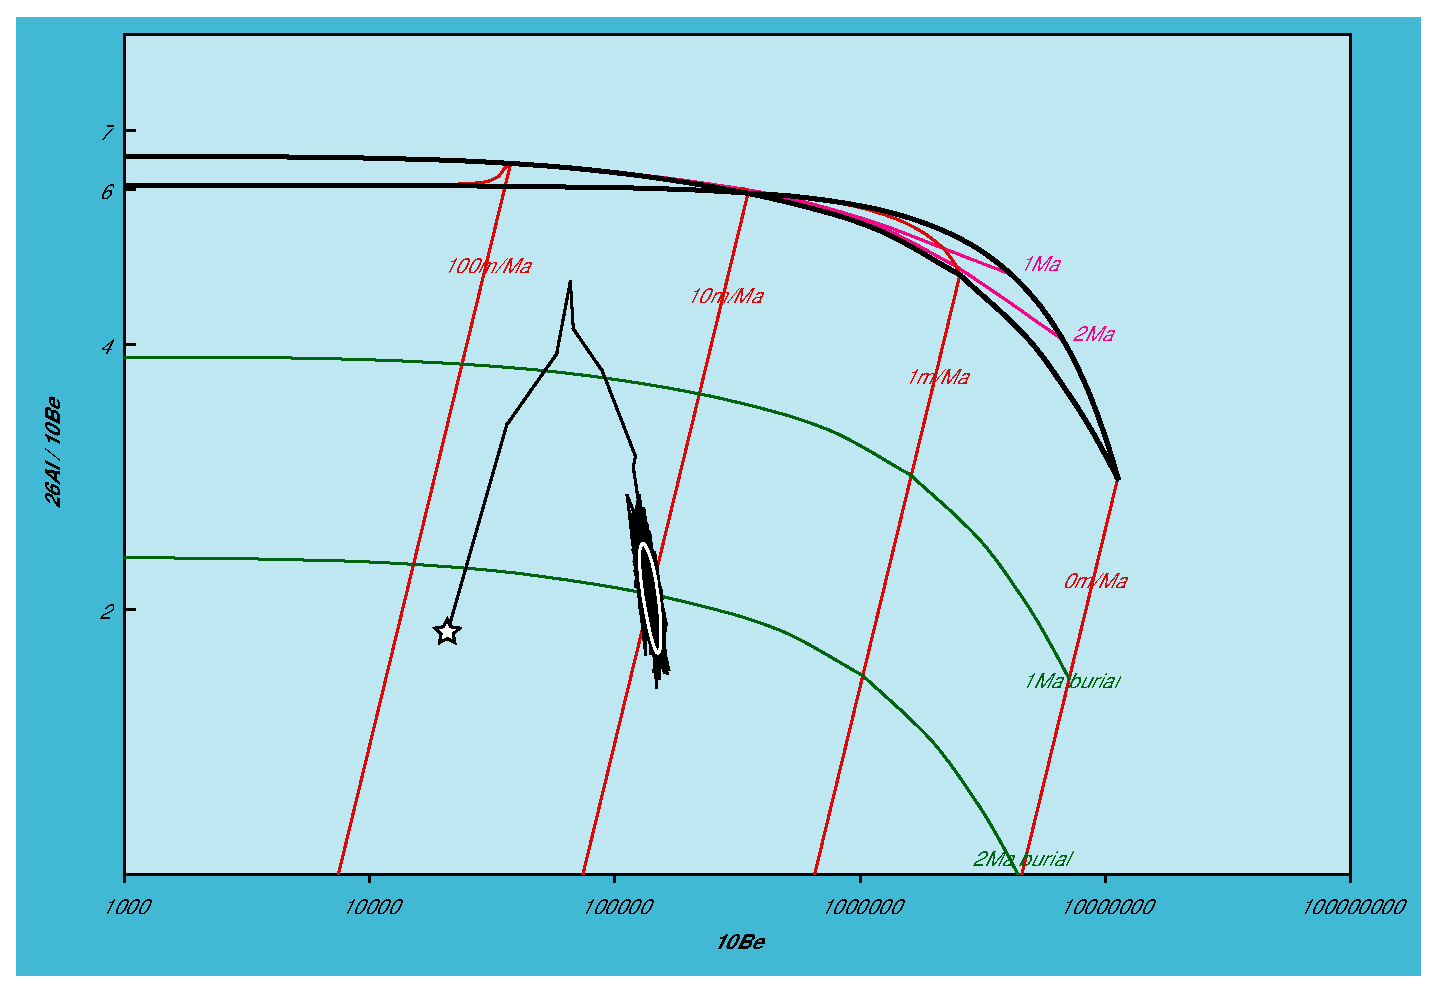
\includegraphics[width=0.7\textwidth]{2006GC001530-f03_orig.eps}
  \caption{
    Starting with  a random  guess (white star)  for the  erosion rate
    ($\epsilon$)  and  burial  age ($\tau$),  the  Metropolis-Hastings
    algorithm quickly  finds the optimal solution.   It then continues
    to randomly  sample the solution space defined  by the measurement
    uncertainties.   The  white ellipse  is  the 2$\sigma$  confidence
    region,   which  corresponds  to   $\sim$90\%  of   the  bivariate
    ($\epsilon$,$\tau$) solution-space.   The black area  contains the
    last 90\% of the 1000  accepted values generated by the algorithm. 
    95\% of  these 900 values  are used to calculate  the simultaneous
    confidence intervals for $\epsilon$~and~$\tau$.}
  \label{fig:metropolisBanana}
\end{figure}

\subsubsection{An {\it a posteriori} modification of the banana plots}\label{sec:Se}

Section    \ref{sec:banana}     discussed    the    construction    of
$^{26}$Al-$^{10}$Be  and $^{21}$Ne-$^{10}$Be  banana  plots.  To  plot
samples  from  different  field  locations (with  different  latitude,
elevation and shielding conditions)  together on the same banana plot,
it is  necessary to  scale the TCN  concentrations to SLHL.   In other
words,  each  TCN concentration  must  be  divided  by an  appropriate
scaling  factor,  the  so-called  ``effective scaling  factor''  S$_e$
(Equation \ref{eq:Se}):

\begin{equation}
  \label{eq:ScalingN}
  S_e = \frac{N_{meas}}{N_{SLHL}}
\end{equation}

With  N$_{meas}$ the  measured TCN  concentration, and  N$_{SLHL}$ the
equivalent TCN  concentration which would  be measured had  the sample
been collected from  SLHL.  In the case of  zero erosion, N$_{SLHL}$ =
N$_{meas}$  / (S$_p$ $\times$  S$_t$ $\times$  S$_s$ $\times$  S$_c$). 
This is  no longer  true when $\epsilon$  $>$ 0, because  the relative
contributions of neutron spallation,  slow and fast muons change below
the surface.  This is  the ``fractionation'' effect that was discussed
in    Section   \ref{sec:banana}    and    quantified   by    Equation
\ref{eq:solveSx}.   For  example,  consider   the  case  of  two  high
latitude,  high   elevation  samples,  one   with  negligible  erosion
($\epsilon$=0)  and  one   with  non-zero  erosion  ($\epsilon$$>$0).  
Because the  relative importance of neutron  spallation increases with
decreasing erosion rate, and  neutrons are more important (relative to
muons)  at   higher  elevations,  S$_e$   will  be  greater   for  the
zero-erosion  than for  the  non-zero erosion  case.  CosmoCalc  first
solves Equation \ref{eq:burialSystem} or \ref{eq:ageErosionSystem} for
$\epsilon$  and   $\tau$  or  t,  whichever  fits   the  measured  TCN
concentrations   best.   Plugging   these   solutions  into   Equation
\ref{eq:Nbanana}  yields the  equivalent  TCN concentration  at SLHL.  
S$_e$ is then given by Equation \ref{eq:ScalingN}.

\section{Converters}\label{sec:converter}

Section \ref{sec:scaling} discussed four different models to scale TCN
production rates from  SLHL to any other location  on Earth. All these
models  have  in common  that  they require  two  columns  of data  in
CosmoCalc:  ``latitude'' and  ``elevation''. They  differ in  how they
quantify these two  pieces of information. The scaling  factors of Lal
(1991) are the only ones that use the actual geographical latitude (in
degrees)  and  elevation (in  meters).   Stone  (2000)  also uses  the
geographical  latitude for  estimating the  latitude effect,  but uses
atmospheric  pressure (in  mbar) for  modeling the  elevation  effect. 
Dunai (2000) uses the  geomagnetic inclination (in degrees) instead of
latitude, and  atmospheric depth (in  g/cm$^2$) instead of  elevation. 
Finally, Desilets et al. (2003, 2006) use cut-off rigidity (in GV) for
the latitude effect and atmospheric depth for the elevation effect.
\\

All  these different  measures of  ``latitude'' and  ``elevation'' are
related  to each  other  and can  be  converted into  each other.   To
facilitate the  comparison of the different methods  and, for example,
reinterpret published literature data,  CosmoCalc provides a series of
easy-to-use conversion tools.

\subsection{Converting different measures of ``elevation''}\label{sec:elevation}

To convert  elevation (z, in m)  to atmospheric pressure  (p, in mbar)
(Iribane and Godson, 1992):

\begin{equation}
  \label{eq:z2p}
  p = p_0 \left(1 - \frac{\beta_0 z}{T_0}\right)^{\frac{g_0}{R_d \beta_0}}
\end{equation}

With p$_0$  the pressure at  sea level, $\beta_0$ the  adiabatic lapse
rate,  T$_0$ the  temperature at  sea level,  g$_0$  the gravitational
constant  and  R$_d$ the  universal  gas  constant.   In the  standard
atmospheric  model, $\beta_0$  = 6.5  K/km, g$_0$  =  9.80665 m/s$^2$,
p$_0$ = 1013.25  mbar and T$_0$ = 288.15 K.  However, these values are
not valid for  Antarctica, where p$_0$ $\approx$ 989.1  mbar and T$_0$
$\approx$ 250 K.  The  modified Equation \ref{eq:z2p} can be rewritten
as (Stone, 2000):

\begin{equation}
  \label{eq:z2antP}
  p_{ant} = 989.1 e^{-\frac{z}{7588}}
\end{equation}

Atmospheric pressure is converted to atmospheric depth (g/cm$^2$) by:

\begin{equation}
  \label{eq:p2d}
  d = 10 \frac{p}{g_0}
\end{equation}

The reverse conversions are trivial inversions of these equations.

\subsection{Converting different measures of ``latitude''}\label{sec:latitude}

Converting latitude (L, in  degrees) to geomagnetic inclination (I, in
degrees) and back:

\begin{equation}
  \label{eq:l2i}
\mbox{tan I = 2 tan L}
\end{equation}

Converting  latitude to  geomagnetic cut-off  rigidity (in  GV)  for a
geomagnetic  field strength M,  compared to  the 1945  reference value
(M$_0$ = 8.085$\times$10$^2$ A m$^2$):

\begin{equation}
  \label{eq:L2Rc}
  R_c = \sum_{i=1}^{6}\left(e_i + f_i\left(\frac{M}{M_0}\right)\right) L^i
\end{equation}

The default value for M/M$_0$ =  1, but can be changed by clicking the
``Option'' button  of the CosmoCalc  conversion form.  e$_1,...,$e$_6$
and  f$_1,...,$f$_6$ are  defined in  Table  8 of  Desilets and  Zreda
(2003). The reverse operation  of Equation \ref{eq:L2Rc} does not have
an analytical solution and is solved iteratively with Newton's method.

\section{Customizing CosmoCalc}\label{sec:settings}

The interface of  CosmoCalc is very simple because  default values are
set for  most of  the parameters that  occur in the  various equations
discussed  in  this paper  (Table  \ref{tab:defaults}).  This  greatly
reduces the chance that novice users make mistakes when reducing their
TCN data. For  more advanced users, the program  allows nearly all the
parameters to be changed.

\subsection{Specifying the production rate calibration sites} 
\label{sec:calibration}

As mentioned in Section \ref{sec:scaling}, it is very important to use
a consistent  set of  scaling factors for  the unknown sample  and the
production  rate  calibration  site.   Failing  to  do  so  can  cause
significant systematic  errors.  To avoid this,  CosmoCalc defines the
SLHL  production  rates  {\it  implicitly},  by specifying  a  set  of
calibration sites  and their  measured TCN concentrations.   Using the
``Calibration   sites''   form  of   the   ``Settings''  menu,   these
concentrations are  scaled to SLHL  and an average production  rate is
calculated  using   one  of  the   five  scaling  models   of  Section
\ref{sec:scaling}.  CosmoCalc  comes with  a default set  of published
production rate calibrations, some  of which ($^{10}$Be and $^{26}$Al)
were      borrowed      from      Balco     and      Stone      (2007;
\texttt{http://hess.ess.washington.edu/math}).    The  published  data
come from a variety of latitudes and elevations, yielding a presumably
reliable estimate  of the  globally averaged production  rates.  This,
however, is not always the best approach.  For example, if a TCN study
is carried  out in  the vicinity of  one particular  calibration site,
then it makes  more sense to use only this site  to estimate the local
production rate.  Therefore, CosmoCalc offers the user the flexibility
to delete or add calibration sites at will.

\subsection{Changing the relative contributions of different production pathways} \label{sec:F}

Being  based on  the equation  of Granger  and Smith  (2000),  the TCN
production equation  consists of four exponentials:  one for neutrons,
two  for  slow neutrons,  and  one  for  fast neutrons  (see  Equation
\ref{eq:Nage}  and  Section  \ref{sec:age}).  These  exponentials  are
governed  by two  sets  of  parameters: the  fractions  F$_i$ and  the
attenuation lengths  $\Lambda_i$ (for i=0,...,3).   Default values for
$\Lambda_i$,  F$_i$($^{10}$Be) and  F$_i$($^{26}$Al)  were taken  from
Granger and Smith (2000)  (Table \ref{tab:defaults}), but these values
can be changed in the ``Settings'' form.
\\

\begin{table}[here]
  \centering
% Table generated by Excel2LaTeX from sheet 'Sheet1'
\begin{tabular}{llrl}
parameter &     symbol & default value &      units \\
\hline
rock density &    $\rho$ &       2.65 &  g/cm$^3$ \\
decay constant ($^{10}$Be) & $\lambda$($^{10}$Be) &  4.560E-07 & yr$^{-1}$ \\
decay constant ($^{26}$Al) & $\lambda$($^{26}$Al) &  9.800E-07 & yr$^{-1}$ \\
decay constant ($^{36}$Cl) & $\lambda$($^{36}$Cl) &  2.300E-06 & yr$^{-1}$ \\
decay constant ($^{14}$C) & $\lambda$($^{14}$C) &  1.213E-04 & yr$^{-1}$ \\
attenuation length (neutrons) & $\Lambda_0$ &        160 &  g/cm$^2$ \\
attenuation length (slow muons) & $\Lambda_1$ &        738 &  g/cm$^2$ \\
attenuation length (slow muons) & $\Lambda_2$ &       2688 &  g/cm$^2$ \\
attenuation length (fast muons) & $\Lambda_3$ &       4360 &  g/cm$^2$ \\
relative production by neutrons ($^{10}$Be) & F$_0$($^{10}$Be) &  0.9724 & -- \\
relative production by neutrons ($^{26}$Al) & F$_0$($^{26}$Al) &  0.9655 & -- \\
relative production by neutrons ($^{14}$C) & F$_0$($^{14}$C) &    0.83 & -- \\
relative production by neutrons ($^{36}$Cl) & F$_0$($^{36}$Cl) &  0.903 & -- \\
relative production by neutrons ($^{3}$He) & F$_0$($^{3}$He) &    1 & -- \\
relative production by neutrons ($^{21}$Ne) & F$_0$($^{21}$Ne) &  1 & -- \\
relative production by slow muons ($^{10}$Be) & F$_1$($^{10}$Be) & 0.0186 & -- \\
relative production by slow muons ($^{26}$Al) & F$_1$($^{26}$Al) & 0.0233 & -- \\
relative production by slow muons ($^{14}$C) & F$_1$($^{14}$C) &   0.0691 & -- \\
relative production by slow muons ($^{36}$Cl) & F$_1$($^{36}$Cl) & 0.0447 & -- \\
relative production by slow muons ($^{3}$He) & F$_1$($^{3}$He) &   0 & -- \\
relative production by slow muons ($^{21}$Ne) & F$_1$($^{21}$Ne) & 0 & -- \\
relative production by slow muons ($^{10}$Be) & F$_2$($^{10}$Be) & 0.004 & -- \\
relative production by slow muons ($^{26}$Al) & F$_2$($^{26}$Al) & 0.005 & -- \\
relative production by slow muons ($^{14}$C) & F$_2$($^{14}$C) &   0.0809 & -- \\
relative production by slow muons ($^{36}$Cl) & F$_2$($^{36}$Cl) & 0.0523 & -- \\
relative production by slow muons ($^{3}$He) & F$_2$($^{3}$He) &   0 & -- \\
relative production by slow muons ($^{21}$Ne) & F$_2$($^{21}$Ne) & 0 & -- \\
relative production by fast muons ($^{10}$Be) & F$_3$($^{10}$Be) & 0.005 & -- \\
relative production by fast muons ($^{26}$Al) & F$_3$($^{26}$Al) & 0.0062 & -- \\
relative production by fast muons ($^{14}$C) & F$_3$($^{14}$C) &   0.02 & -- \\
relative production by fast muons ($^{36}$Cl) & F$_3$($^{36}$Cl) & 0 & -- \\
relative production by fast muons ($^{3}$He) & F$_3$($^{3}$He) &   0 & -- \\
relative production by fast muons ($^{21}$Ne) & F$_3$($^{21}$Ne) & 0 & -- \\
sea level temperature &     T$_0$ &     288.15 &          K \\
adiabatic lapse rate & $\beta_0$ &        6.5 &       K/km \\
air pressure at sea level &     P$_0$ &    1013.25 &       mbar \\
geomagnetic field intensity relative to 1945 &   M/M$_0$ &          1 &   --         \\
\end{tabular}  
  \caption{Default values of CosmoCalc parameters}
  \label{tab:defaults}
\end{table}

In  addition  to  Equation  \ref{eq:Nage},  several  alternative,  but
similar  looking  TCN ingrowth  equations  exist  in  the literature.  
Schaller et al. (2001, 2002)  use not four but eight exponentials (two
for neutrons, and three for  each slow and fast muons), whereas others
use three (one for each  production mechanism) (e.g., Braucher et al.,
2003; Miller  et al., 2006)  or only one exponential  (neglecting muon
production).  CosmoCalc provides a  separate set of default parameters
for each of these alternatives.  For example, the ingrowth equation of
Schaller et al.  (2002) was  recast in the parameterization of Granger
and Smith  (2000) by a  least squares fit  of a virtual  depth profile
(Figure \ref{fig:granger2schaller}).

\begin{figure}[h]
  \centering 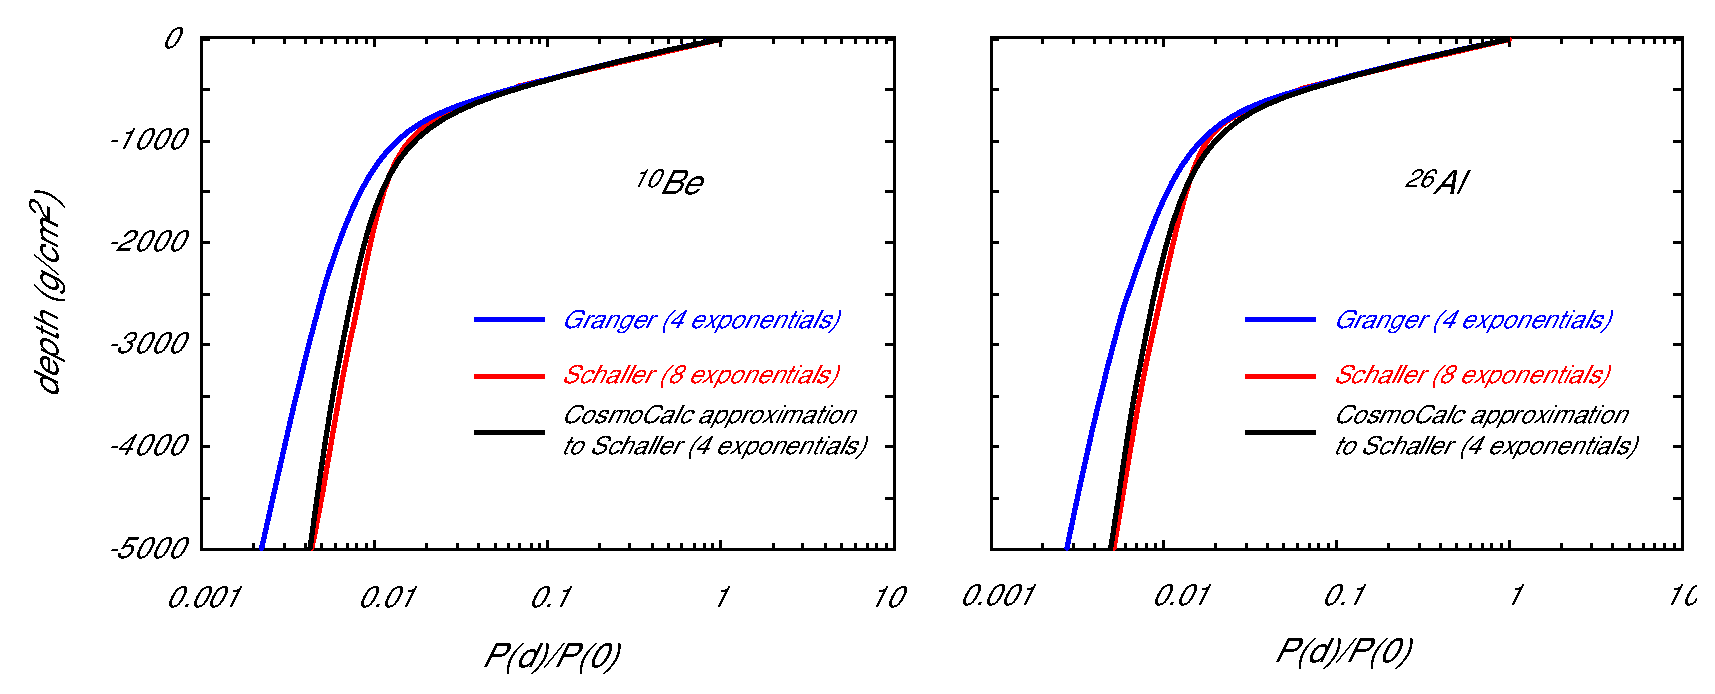
\includegraphics[width=\textwidth]{2006GC001530-f04_orig.eps}
  \caption{
    To implement the  TCN ingrowth equation of Schaller  et al. (2001,
    2002),  CosmoCalc uses  a least  squares fit  of the  TCN ingrowth
    equation  of  Granger and  Smith  (2000)  to  a ``virtual''  depth
    profile defined by this alternative ingrowth equation.}
  \label{fig:granger2schaller}
\end{figure}

\section{How to report data reduced with CosmoCalc}

CosmoCalc was designed  to be a user-friendly program  for both novice
and advanced users of TCN  methods. Nearly every function comes with a
set of  options which allow the  user to change the  default values of
various parameters (Section \ref{sec:settings}).  Although CosmoCalc's
flexibility should  be considered a positive feature,  a danger exists
that his may  lead to confusion.  Therefore, it  is important that the
data-reduction method is well  documented when reporting results. Here
is an example:
\\

``{\it  Ages were  calculated  with CosmoCalc  1.0 (Vermeesch,  2007),
  using  Dunai  (2000) scaling  factors  and  default  values for  all
  parameters with the following  exceptions: $\rho$ = 3.5 g/cm$^3$ and
  $\lambda$($^{10}$Be) = 5.17$\times$10$^{-7}$yr$^{-1}$.}''
\\

Clearly indicating  the version number is  important because CosmoCalc
will be updated in the future to keep track of new developments in TCN
geochronology.   Older  versions will  always  be  available from  the
CosmoCalc  website (\texttt{http://cosmocalc.googlepages.com}).  Users
with useful suggestions for  improvements should feel free contact the
author by emailing to \texttt{cosmocalc@gmail.com}.
\\

{\it Acknowledgments.}  The author is financially supported by a Marie
Curie Fellowship of the European Union (CRONUS-EU network, RTN project
reference  511927).  Many thanks  to Dr.   Naki Ak\c{c}ar  for testing
beta-versions  of  CosmoCalc   and  making  useful  suggestions  which
simplified the user interface and made the program more user-friendly,
and to two anonymous reviewers for constructive comments.

\clearpage

\section*{References}

\begin{description}
  
\item Balco,  G., and J.O.H.  Stone, A  simple, internally consistent,
  and easily accessible means  of calculating surface exposure ages or
  erosion  rates  from $^{10}$Be  and  $^{26}$Al  measurements, {\it  Quaternary
    Geochronology}, (in preparation).
  
\item Bierman, P.R., K.A. Marsella,  C. Patterson, P.T.  Davis, and M. 
  Caffee,   Mid-Pleistocene    cosmogenic   minimum-age   limits   for
  pre-Wisconsian  glacial  surfaces   in  southwestern  Minnesota  and
  southern   Baffin  island:   a  multiple   nuclide   approach,  {\it
    Geomorphology, 27} (1-2), 25-39, 1999.
  
\item Braucher, R., E.T. Brown,  D.L.  Bourles, and F.  Colin, In situ
  produced  $^{10}$Be  measurements   at  great  depths:  implications  for
  production  rates by fast  muons, {\it  Earth and  Planetary Science
    Letters, 211}, 251-258, 2003.

\item Brown,  E.T., T.W.  Trull, P.  Jean-Baptiste,  G.  Raisbeck,  D. 
  Bourles,  F.   Yiou,  and  B.  Marty,  Determination  of  cosmogenic
  production  rates  of  $^{10}$Be,  $^3$He  and $^3$H  in  water,  {\it  Nuclear
    Instruments  and Methods  in  Physics Research  B, 172},  802-805,
  2000.

\item Chayes, F., On ratio correlation in petrography, {\it Journal of
    Geology, 57} (3), 239-254, 1949.
  
\item Desilets, D., and M. Zreda, Spatial and temporal distribution of
  secondary cosmic-ray nucleon intensities and applications to in situ
  cosmogenic dating,  {\it Earth and Planetary  Science Letters, 206},
  21-42, 2003.
  
\item Desilets, D.,  M. Zreda, and T. Prabu,  Extended scaling factors
  for in  situ cosmogenic nuclides: New measurements  at low latitude,
  {\it Earth and Planetary Science Letters, 246}, 265-276, 2006.
  
\item Dunai,  T.J., Scaling  factors for production  rates of  in situ
  produced  cosmogenic nuclides: a  critical reevaluation,  {\it Earth
    and Planetary Science Letters, 176}, 157-169, 2000.
  
\item Dunai,  T.J., Influence of secular variation  of the geomagnetic
  field on  production rates of in situ  produced cosmogenic nuclides,
  {\it Earth and Planetary Science Letters, 193}, 197-212, 2001.
  
\item Dunai,  T.J., and Wijbrans J.R., Long-term  $^3$He production rates
  (152  ka -  1.35 Ma)  from 40Ar/39Ar  dated basalt  flows  at 29$^o$
  latitude, {\it  Earth and Planetary Science  Letters, 176}, 147-156,
  2000.
  
\item Fabel, D., A.P. Stroeven,  J. Harbor, J.  Kleman, D. Elmore, and
  D.   Fink,  Landscape preservation  under  Fennoscandian ice  sheets
  determined  from in  situ produced  $^{10}$Be  and $^{26}$Al,  {\it Earth  and
    Planetary Science Letters, 201}, 397-406, 2002.
  
\item  Graham, I.J.,  Barry, B.J.,  Ditchburn, R.G.,  Whitehead, N.E.,
  Zondervan, A.,  Direct measurement  of cosmogenic production  of 7Be
  and $^{10}$Be in water targets in the southern hemisphere, {\it Earth and
    Planetary Science Letters} (in preparation)
  
\item  Granger, D.E., and  A.L. Smith,  Dating buried  sediments using
  radioactive  decay and muogenic  production of  $^{26}$Al and  $^{10}$Be, {\it
    Nuclear  Instruments  and Methods  in  Physics  Research B,  172},
  822-826, 2000.

\item Granger,  D.E., C.S.  Riebe,  J.W.  Kirchner, and  R.C.  Finkel,
  Modulation of erosion on  steep granitic slopes by boulder armoring,
  as revealed  by cosmogenic $^{26}$Al  and $^{10}$Be, {\it Earth  and Planetary
    Science Letters, 186}, 269-281, 2001.
  
\item Granger, D.E., and P.F.  Muzikar, Dating sediment burial with in
  situ-produced   cosmogenic   nuclides:   theory,   techniques,   and
  limitations,  {\it  Earth   and  Planetary  Science  Letters,  188},
  269-281, 2001.

\item Gosse, J.C., E.B. Evenson,  J. Klein, B. Lawn, and R. Middleton,
  Precise  cosmogenic  $^{10}$Be  measurements  in western  North  America:
  Support for a global Younger Dryas cooling event, {\it Geology, 23},
  877-880, 1995.

\item Gosse,  J.C., and F.M. Phillips, Terrestrial  in situ cosmogenic
  nuclides: theory  and application, {\it  Quaternary Science Reviews,
    20}, 1475-1560, 2001.
  
\item Heisinger, B.,  D. Lal, A.J. Jull, S. Ivy-Ochs,  S. Neumaier, K. 
  Knie, V.  Lazarev, and  E.  Nolte, Production of selected cosmogenic
  radionuclides  by muons:  1. Fast  Muons, {\it  Earth  and Planetary
    Science Letters, 200}, 345-355, 2002.
  
\item Heisinger, B., D. Lal, A.J.   Jull, P.W. Kubik, S.  Ivy-Ochs, K. 
  Knie, and E. Nolte,  Production of selected cosmogenic radionuclides
  by muons:  2. Capture  of negative muons,  {\it Earth  and Planetary
    Science Letters, 200}, 357-369, 2002.
  
\item Iribane, J.V., and  W.L. Godson, Atmospheric Thermodynamics, 259
  pp., D. Reidel, Dordrecht, 1992.
  
\item  Kubik, P.W.,  S.   Ivy-Ochs, J.   Masarik,  M.  Frank,  and C.  
  Schl\"{u}chter,  $^{10}$Be  and $^{26}$Al  production  rates  deduced from  an
  instantaneous  event   within  the  dendro-calibration   curve,  the
  landslide  of K\"{o}fels,  \"{O}tz  Valley Austria,  {\it Earth  and
    Planetary Science Letters, 161}, 231-241, 1998.

\item Kurz, M.D., Cosmogenic  helium in terrestrial igneous rock, {\it
    Nature, 320}, 435-439, 1986.
  
\item Lifton, N.A., J.W. Bieber,  J.M. Clem, M.L. Dulding, P. Evenson,
  J.E. Humble, and R.  Pyle, Addressing solar modulation and long-term
  uncertainties  in   scaling  secondary  cosmic  rays   for  in  situ
  cosmogenic  nuclide applications, {\it  Earth and  Planetary Science
    Letters, 239}, 140-161, 2005.

\item  Lal, D.,  Cosmic  ray  labeling of  erosion  surfaces: in  situ
  nuclide  production  rates  and   erosion  models,  {\it  Earth  and
    Planetary Science Letters, 104}, 424-439, 1991.
  
\item Metropolis,  N., A.W. Rosenbluth, M.N.  Rosenbluth, A.H. Teller,
  and  E. Teller, Equations  of state  calculations by  fast computing
  machines, {\it Journal of Chemical Physics, 21}, 1087-192, 1953.
  
\item Miller, G.H., J.P. Briner, N.A. Lifton, and R.C. Finkel, Limited
  ice-sheet  erosion and  complex exposure  histories derived  from in
  situ cosmogenic $^{10}$Be, $^{26}$Al, and 14C on Baffin Island, Arctic Canada,
  {\it Quaternary Geochronology, 1}, 74-85, 2006.

\item Niedermann, S., T. Graf, J.S.  Kim, C.P. Kohl, K.  Marti, and K. 
  Nishiizumi, Cosmic-ray produced $^{21}$Ne in terrestrial quartz: the neon
  inventory  of  Sierra  Nevada   quartz  separates,  {\it  Earth  and
    Planetary Science Letters, 125}, 341-355, 1994.

\item Nishiizumi, K., D. Lal, J. Klein, R. Middleton, and J.R. Arnold,
  Production of $^{10}$Be and $^{26}$Al  by cosmic rays in terrestrial quartz in
  situ and implications for erosion rates, {\it Nature, 319}, 134-135,
  1986.
  
\item Nishiizumi, K.,  E. L.  Winterer, et al.   Cosmic ray production
  rates of $^{10}$Be and $^{26}$Al in quartz from glacially polished rocks. {\it
    Journal of Geophysical Research, 94}, 17907-17915, 1989.

\item Nishiizumi, K., C.P. Kohl,  J.R. Arnold, J.  Klein, D. Fink, and
  R. Middleton, Cosmic ray produced  $^{10}$Be and $^{26}$Al in Antarctic rocks:
  exposure  and  erosion history,  {\it  Earth  and Planetary  Science
    Letters, 104}, 440-454, 1991.
  
\item Nishiizumi, K., R.C. Finkel, J. Klein, and C.P. Kohl, Cosmogenic
  production  of  $^7$Be and  $^{10}$Be  in  water  targets, {\it  Journal  of
    Geophysical Research., 101}, 22225-22232, 1996.
  
\item Partridge,  T.C., D.E.  Granger, M.W.  Caffee,  and R.J. Clarke,
  Lower  Pliocene  hominid remains  from  Sterkfontein, {\it  Science,
    300}, 607-612, 2003.
  
\item Phillips,  F.M., B.D.  Leavy, N.O.  Jannik, D. Elmore,  and P.W. 
  Kubik, The  accumulation of cosmogenic  Chlorine in rocks:  a method
  for surface exposure dating, {\it Science, 231}, 41-43, 1986.
  
\item  Phillips,  F.M.,  and   M.A.  Plummer,  CHLOE:  A  program  for
  interpreting in  situ cosmogenic  nuclide data for  surface exposure
  dating and erosion studies, {\it Radiocarbon, 38}, 98, 1996.
  
\item  Pigati,   J.S.,  and  N.A.   Lifton,   Geomagnetic  effects  on
  time-integrated  cosmogenic nuclide production  with emphasis  on in
  situ 14C and  $^{10}$Be, {\it Earth and Planetary  Science Letters, 226},
  193-205, 2004.

\item Sch\"{a}fer,  J.M., S. Ivy-Ochs,  R. Wieler, I. Leya,  H.  Baur,
  G.H.  Denton,  and C.  Schl\"{u}chter, Cosmogenic  noble gas studies
  in the oldest  landscape on earth: surface exposure  ages of the Dry
  Valleys, Antarctica, {\it Earth and Planetary Science Letters, 167},
  215-226, 1999.
  
\item Schaller, M., F. von  Blanckenburg, N.  Hovius, and P.W.  Kubik,
  Large-scale erosion rates  from in situ-produced cosmogenic nuclides
  in  European  river  sediments,  {\it Earth  and  Planetary  Science
    Letters, 188}, 441-458, 2001.
  
\item Schaller, M., F. von Blanckenburg, A. Veldkamp, L.A. Tebbens, N.
  Hovius,  and P.W.   Kubik, A  30000yr record  of erosion  rates from
  cosmogenic  $^{10}$Be in  Middle Europe  river terraces,  {\it  Earth and
    Planetary Science Letters, 204}, 307-320, 2002.
  
\item  Staudacher,  T., and  C.J.   All\`{e}gre,  Ages  of the  second
  caldera of Piton de la Fournaise volcano (R\'{e}union) determined by
  cosmic ray  produced $^3$He and $^{21}$Ne, {\it  Earth and Planetary
    Science Letters, 119}, 395-404, 1993.
  
\item Stone,  J.O., G.L.  Allan,  L.K.  Fifield, and  R.G.  Cresswell,
  Cosmogenic chlorine-36  from calcium spallation,  {\it Geochimica et
    Cosmochimica Acta, 60}, 555-561, 1996.

\item Stone, J., Air pressure  and cosmogenic isotope production, 
  {\it Journal of Geophysical Research, 105}, 23753-23759, 2000.
  
\item Tarantola,  A., {\it Inverse  problem theory}, 342  pp., Society
  for Industrial and Applied Mathematics, 2004.

\end{description}

\end{document}